\parindent=0em
\subsection{Magic Leap One}
\noindent

El dispositivo \textit{Magic Leap One}\textsuperscript{\ref{magicLeaponeFotterSpecs}} fue lanzado al mercado el 8 de Agosto de 2018 de manos de la compañía Magic Leap a un precio inicial de 2,295 dólares exclusivamente en Chicago, Los Ángeles, Miami, Nueva York, San Francisco y Seattle .\\

En el ámbito técnico este casco destaca por su ligero peso de 316 gramos frente a los 566 gramos de la HoloLens 2 (sección \ref{HoloLens2Dispositivo}), posee un sistema 6DoF para el tracking, conectividad vía Bluetooth 4.2, WiFi o USB tipo C.\\

\begin{figure}[htbp]
\centering
    \hspace{-4mm}
    \begin{minipage}{0.5\textwidth}
        \centering
        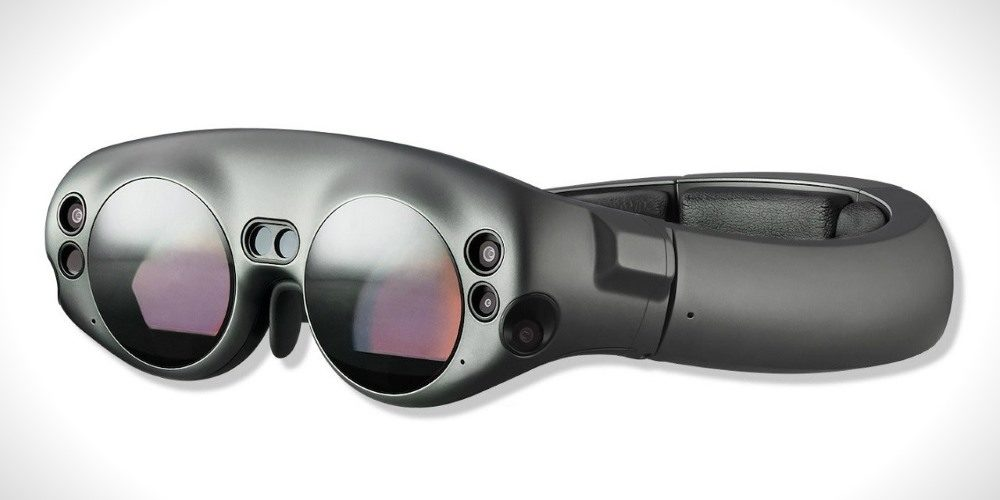
\includegraphics[scale=0.8]{Images/Estado del arte/magicleapone1.jpg}\\
        (a) Vista del casco completo
    \end{minipage}
    \begin{minipage}{0.5\textwidth}
        \centering
        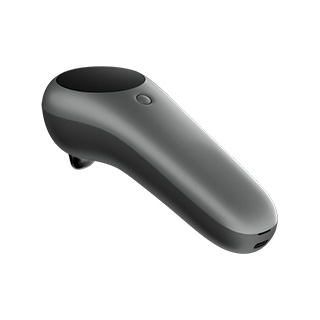
\includegraphics[scale=0.3]{Images/Estado del arte/magicleapone2.jpg}\\
       (b) Vista del mando
    \end{minipage}\\
    \caption{Dispositivo completo de las Magic Leap One\textsuperscript{\ref{magicLeaponeFotterImages}}.}
    \label{fig:vistasMagicLeapnOne}
\end{figure}

Por otro lado, utiliza una CPU (Unidad Central de Procesamiento) dos núcleos Denver 2.0 64-bit y cuatro núcleos ARM Cortex A57 64-bit, una Nvidia Pascal de 256 núcleos CUDA para la GPU (Unidad de Procesamiento Gráfico), tiene 128 Gigabytes como capacidad de almacenamiento y, por último, una batería de litio recargable que permite un uso continuado de 3 horas. 


%https://www.businessinsider.com/magic-leap-one-creator-edition-price-specifications-battery-life-release-date-2018-8?IR=T


\footnotetext[1]{
\label{magicLeaponeFotterSpecs}{Especificaciones obtenidas de \url{https://www.businessinsider.com/magic-leap-one-creator-edition-price-specifications-battery-life-release-date-2018-8?IR=T}.}}

\footnotetext[1]{
\label{magicLeaponeFotterImages}{Imágenes sacadas de \url{https://www.estiloextra.net/magic-leap-one-las-nuevas-y-prometedoras-gafas-de-realidad-aumentada/}.}}
